\documentclass[12pt]{article}

\usepackage[margin=0.5in]{geometry}
\usepackage{amsmath}
\usepackage{tikz}
\usepackage{hyperref}
\usepackage{multicol}


\newcommand{\ds}{\displaystyle}

\begin{document}
\pagestyle{empty}
\subsubsection*{Midterm 2 Review Problems \hfill Math 140 }
\textit{These are suggested review problems similar to what might be on Midterm 2. Included with each problem is a link to a video where you can see how the problem is solved. I didn't make the videos, they are all  available online.}

\begin{enumerate}

%\item Solve $x^2 + 2x - 24 > 0$.
%\vfill 
%\hfill  \url{https://youtu.be/E9UsqBX1BPw}
%\hrule 
%
%\item Solve $\ds 2x^3 - 98x \le 0$.
%\vfill
%\hfill \url{https://youtu.be/E9UsqBX1BPw?t=282}
%\hrule
%
%\item Solve $\ds \frac{1}{x-2} > \frac{-1}{x^2 - 7x + 10}$.  
%\vfill
%\hfill \url{https://youtu.be/E9UsqBX1BPw?t=517}
%\hrule

\item Calculate the following derivatives.
\begin{enumerate}
\begin{multicols}{2}
\item $\dfrac{d}{dx} e^{5x+3}$ 
\item $\dfrac{d}{dx} e^{x^2}$
\end{multicols}
\end{enumerate}
\vfill
\hfill \url{https://youtu.be/yg_497u6JnA}
\hrule

\item Calculate the following logarithms.
\begin{enumerate}
\begin{multicols}{3}
\item $\log_3(81)$ 
\item $\log_2(64)$
\item $\log_{100}(1)$
\end{multicols}
\end{enumerate}
\vfill
\hfill \url{https://youtu.be/Z5myJ8dg_rM}
\hrule

\item Write each expression as a single natural logarithm using the properties of logarithms. 
\begin{enumerate}
\begin{multicols}{2}
\item $3\ln 10 - \ln 8$ 
\item $2 \ln 5 + 4 \ln 2 + \ln(5y)$
\end{multicols}
\end{enumerate}
\vfill
\hfill \url{https://youtu.be/wRXdiePi5-0}
\hrule


\item Solve $7+3 \ln x = 5$. 
\vfill
\hfill \url{https://youtu.be/vTqzK32bDfE}
\hrule 


\newpage
\item Solve $5e^{-3x} + 1 = 11$.
\vfill
\hfill \url{https://youtu.be/YY2CXOHpuxA}
\hrule

%\item At an annual rate of growth of 3.8\%, how long (exactly) does it take to double an investment if nothing else is added to the account along the way? 
%\vfill
%\hfill \url{https://youtu.be/iB3xENjuxmI}
%\hrule


\item Find the derivative of $\ds f(x) = \ln\left( \frac{x+5}{x-1} \right)$. Hint: Use the properties of logarithms to simplify $f(x)$ before taking the derivative.
\vfill
\hfill \url{https://youtu.be/R2JsjJyr0ck}
\hrule



\item Find the derivative of $\ds y = \frac{2}{x^3}$. 
\vfill
\hfill \url{https://youtu.be/ETL_-_Vj_A0}
\hrule


\item Let $f(x) = \sqrt[3]{x}$. Find $f'(x)$.
\vfill
\hfill \url{https://youtu.be/H-v4oraDjuM?t=73}
\hrule

\newpage
\item Find the derivative of $\ds f(x) = \frac{5x+2}{3x-4}$.
\vfill
\hfill \url{https://youtu.be/BF4e2vbmGkk}
\hrule


\item Calculate $\ds \frac{d}{dx} (x^2 - 2)(7x^3+5)$.
\vfill
\hfill \url{https://youtu.be/8Qw2aPjqW9c}
\hrule

\item Find $\ds \frac{d}{dx} \sqrt{ 3x^2 - x}$.
\vfill
\hfill \url{https://youtu.be/IiBC4ngwH6E}
\hrule


\item Suppose that the total cost for a company to produce $x$ machines is $C(x) = 1100 + 140x - 0.2x^2$. Find the marginal cost $C'(x)$ when 105 machines are produced. 
\vfill
\hfill \url{https://youtu.be/RN0BTZ46Knk}
\hrule 


\item Where does the function $f(x) = x^3 - 6x^2 + 15$ have a horizontal tangent line? 
\vfill
\hfill \url{https://youtu.be/aNfoxbMUOHk}
\hrule

\newpage
\item Let $f(x) = x^3 - 6x^2 + x - 5$.  Find the equation of the tangent line to $f(x)$ when $x = 1$.  
\begin{flushright}
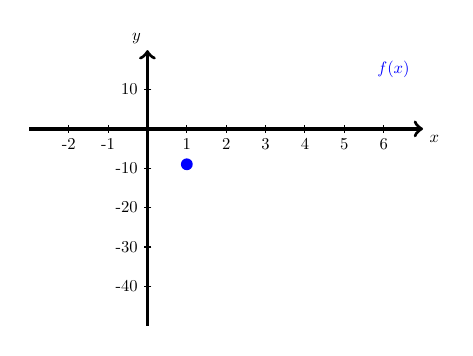
\begin{tikzpicture}[scale=0.5]
\draw[very thick,->] (-3,0) -- (7,0) node[below right,scale=0.6] {$x$};
\draw[very thick,->] (0,-5) -- (0,2) node[above left, scale=0.6] {$y$};
\draw[very thick,color=blue] plot[domain=-2.1:6.2,samples=400] function {(x**3-6*(x**2)+x-5)/10};
\fill[blue] (1,-0.9) circle (0.15);
\foreach \y in {-4,-3,-2,-1,1} {
  \draw (0.1,\y) -- (-0.1,\y) node[left,scale=0.6] {\y0};
}
\foreach \x in {-2,-1,1,2,3,4,5,6} {
  \draw (\x,0.1) -- (\x,-0.1) node[below,scale=0.6] {\x};
}
\draw[blue] (6.25,1.5) node[scale=0.6] {$f(x)$};

\end{tikzpicture}
\end{flushright}
\hfill \url{https://youtu.be/j9FDoYNxZlw}
\hrule






\item Suppose the profit for a bicycle manufacturer is $P(x) = 0.0002 x^3 + 10x$ where $x$ is the number of bicycles they sell.  Find the derivative $P'(x)$ and use it to estimate the marginal profit when $x=100$. 

\vfill
\hfill \url{https://youtu.be/IB-2Umkiok8}
\hrule


\item Find the intervals where $f(x) = 2+3x^2 - x^3$ is concave up and the intervals where it is concave down.  Also, find the inflection points of $f(x)$.  
\vfill
\hfill \url{https://youtu.be/c1N8zyVhWxM}
\hrule

%\item Find the intervals where $h(x) = (x^2-1)^3$ is concave up and the intervals where it is concave down.
%\vfill
%\hfill \url{https://youtu.be/c1N8zyVhWxM?t=183}
%\hrule

\item The kinetic energy of an object is $E = \frac{1}{2} m v^2$ where $m$ is its mass and $v$ is its velocity.  Suppose that a rock has a mass of 2 kilograms and is falling so that its velocity is increasing at a rate of 9 meters per second every second (i.e., $\dfrac{dv}{dt} = 9$).  Use the chain rule to find the rate of change in the rock's kinetic energy with respect to time at the instant when the rock's velocity is 5 meters per second.  
\vfill
\hfill \url{https://youtu.be/NA-Ri4LJPaY}
\hrule 



\end{enumerate}
\end{document}
